\chapter{ทฤษฎีความรู้และงานที่เกี่ยวข้อง}

% \emph{หัวข้อต่าง ๆ ในแต่ละบทเป็นเพียงตัวอย่างเท่านั้น หัวข้อที่จะใส่ในแต่ละบทขึ้นอยู่กับโปรเจคของนักศึกษาและอาจารย์ที่ปรึกษา}

% ตัวอย่างการใส่อ้างอิงที่มา -> \cite{hypersense} ถ้าต้องการใส่แหล่งอ้างอิงมากกว่า 1 ให้ทำดังนี้ -> \cite{hypersense,bworld}
% อธิบายทฤษฎี องค์ความรู้หลักที่ใช้ในงาน งานวิจัยที่นำมาใช้ในโครงงาน หรือเปรียบเทียบผลิตภัณฑ์ที่มีอยู่ในท้องตลาด\cite{bworld}
% Explain theory, algorithms, protocols, or existing research works and tools related to your work.

\section{ทฤษฎีที่เกี่ยวข้อง}
\subsection{Human Computer Interaction (HCI)}
การปฏิสัมพันธ์ระหว่างมนุษย์และคอมพิวเตอร์ (HCI) หมายถึงการศึกษาและออกแบบ
วิธีการในการสร้างปฏิสัมพันธ์ระหว่างมนุษย์และคอมพิวเตอร์ได้อย่างลื่นไหลและ
ได้รับประสบการณ์ที่ดี แม้ว่าคอมพิวเตอร์ในปัจจุบันจะเป็นเครื่องมือที่มีความสามารถสูง 
แต่เพื่อให้ผู้ใช้สามารถใช้งานและเข้าถึงข้อมูลได้อย่างมีประสิทธิภาพ ตัวหลักการของ HCI 
จะทำหน้าที่ออกแบบการปฏิสัมพันธ์โดยมองจากมุมมองของมนุษย์และผู้ใช้ที่เป็นกลุ่มเป้าหมาย 
และทำให้ดีขึ้นกว่าเดิม
\par การศึกษาของ HCI เน้นไปที่การเข้าใจความต้องการของผู้ใช้ 
การออกแบบอินเตอร์เฟซที่ใช้งานง่ายและมีประสิทธิภาพ การทดสอบและปรับปรุงการใช้งาน 
การทำให้ผู้ใช้มีประสิทธิภาพในการติดต่อสื่อสารกับเทคโนโลยี 
และการวิจัยเกี่ยวกับปัญหาที่เกี่ยวข้องกับการปฏิสัมพันธ์ระหว่างมนุษย์และคอมพิวเตอร์ \\
\textbf{การนำไปใช้งาน} : ทางคณะผู้จัดทำได้นำ HCI ที่เป็นศาสตร์ที่สำคัญ
ในการพัฒนาเว็บแอปพลิเคชันให้ใช้งานง่ายและมีประสิทธิภาพมากขึ้น 
การประยุกต์ใช้ HCI กับโปรเจ็คเว็บแอปพลิเคชันจะช่วยให้ผู้ใช้สามารถใช้งานแอปพลิเคชั่น
ได้อย่างสะดวกและมีประสิทธิภาพมากขึ้น
\subsection{Design Thinking}
กระบวนการคิดเชิงออกแบบ (Design Thinking) 
เป็นเครื่องมือที่ใช้ในการคิดเพื่อแก้ไขปัญหาอย่างเป็นระบบและมีประสิทธิภาพ 
และจะเน้นไปที่การแก้ไขปัญหาของกลุ่มเป้าหมายเป็นหลัก (User-Centered) 
โดยกระบวนการคิดเชิงออกแบบจะแบ่งเป็นทั้งหมด 5 ช่วง ได้แก่
\begin{figure}[!h]\centering
    \setlength{\fboxrule}{0.2mm} % can define this in the preamble
    \setlength{\fboxsep}{0.5cm}
    \fbox{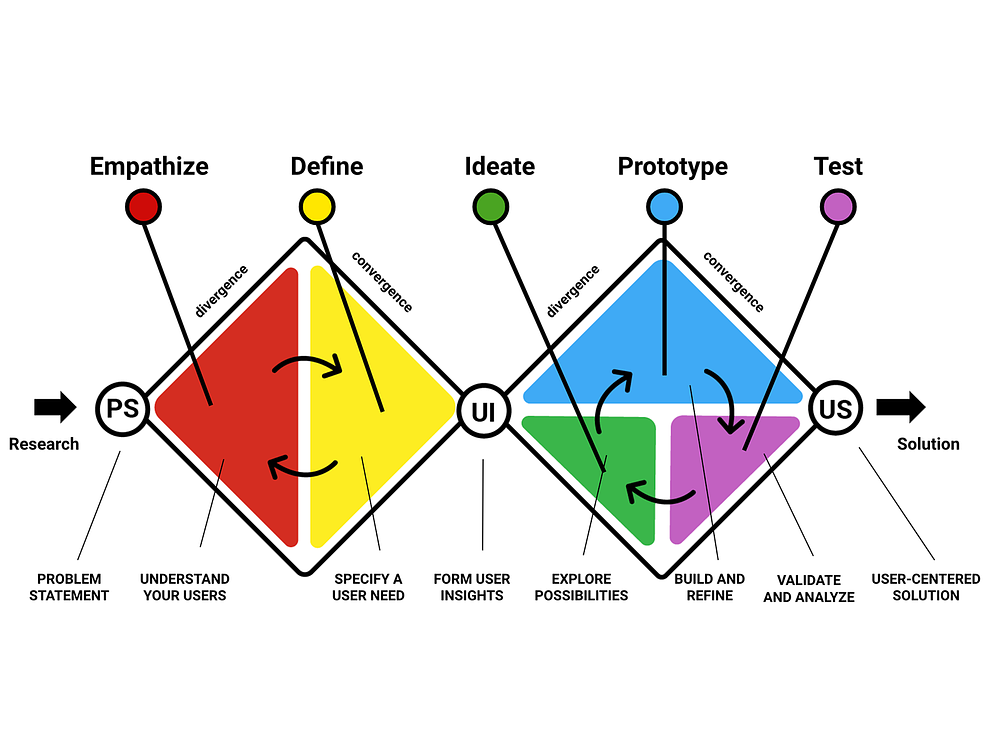
\includegraphics[width=5cm]{./figure/figure_designThinking.png}}
    \caption{ขั้นตอนกระบวนการคิดเชิงออกแบบ}\label{fig:model6}
\end{figure}
\begin{enumerate}
    \item \textbf{Empathize} เป็นการทำความเข้าใจปัญหาที่เกิดขึ้นของกลุ่มเป้าหมายจาก
    การตั้งสมมุติฐาน การสัมภาษณ์กลุ่มเป้าหมาย หรือการสังเกตุพฤติกรรม เป็นต้น
    \item \textbf{Define} นำข้อมูลจากการสัมภาษณ์กลุ่มเป้าหมายมาวิเคราะห์เพื่อ
    กำหนดความต้องการของกลุ่มเป้าหมายให้ชัดเจน
    \item \textbf{Ideate} การระดมสมองเพื่อหาวิธีการแก้ไขปัญหาจากจุดเจ็บปวด 
    (Pain Point) ของกลุ่มเป้าหมายอย่างมีประสิทธิภาพ ตรงประเด็น 
    และให้สามารถใช้งานง่ายที่สุด
    \item \textbf{Prototype} เป็นการสร้างแบบจำลองของวิธีการแก้ไขปัญหาเพื่อ
    ที่จะสามารถนำไปทดสอบกับกลุ่มเป้าหมายได้
    \item \textbf{Test} นำแบบจำลองที่สร้างขึ้นมาทดสอบกับกลุ่มเป้าหมาย 
    เพื่อนำมาปรับปรุงแก้ไขเพื่อให้คำตอบได้อย่างมีประสิทธิภาพมากที่สุด
\end{enumerate}
\textbf{การนำไปใช้งาน} : ทางคณะผู้จัดทำได้นำกระบวนการคิดเชิงออกแบบ 
(Design Thinking) มาประยุกต์ใช้กับโปรเจ็ค ทำให้ได้เว็บแอปพลิเคชันที่ตอบโจทย์
และสามารถใช้งานได้จริง โดยเน้นการเข้าใจผู้ใช้เป็นศูนย์กลาง (User Centric) 
ผ่านการทดลองและทดสอบกับผู้ใช้อย่างต่อเนื่อง
\subsection{MVC Structure}
เฟรมเวิร์กสำหรับการออกแบบสถาปัตยกรรมระบบต่าง ๆ ด้วยหลักการ Design pattern 
ที่จะแยกส่วนระบบการทำงานเป็น 3 ส่วน โดยมีหน้าที่ชัดเจนในแต่ละส่วน ดังนี้
\begin{enumerate}
    \item \textbf{Model} เป็นส่วนที่มีหน้าที่ในการคำนวณตรรกะเชิงข้อมูล เช่น รับส่งข้อมูลกับฐานข้อมูลของระบบ รวมไปถึงจัดการกับข้อมูลก่อนส่งไปสู่ระบบอื่น ๆ โดยส่วน Model นี้ จะตอบรับคำขอจากส่วน Controller เป็นหลัก
    \item \textbf{View} เป็นส่วนสำหรับคำนวณตรรกะในส่วนปฏิสัมพันธ์ผู้ใช้ ซึ่งจะส่งผลต่อสิ่งที่จะนำไปแสดงผลให้ผู้ใช้เห็นทางสายตาโดยตรง หากต้องมีการใช้ข้อมูลจากฐานข้อมูล ส่วน View นี้จะติดต่อขอข้อมูลจากส่วน Controller ก่อน
    \item \textbf{Controller} ส่วนที่ใช้สำหรับติดต่อกับระบบทั้งหมดในโครงสร้าง มีหน้าที่ควบคุมการไหลของเส้นคำขอในซอฟต์แวร์ และคำนวณตรรกะเชิงธุรกิจเท่านั้น หากต้องการใช้ข้อมูลจากฐานข้อมูล ก็จะใช้งานระบบส่วน Model และหากต้องการคำนวณส่วนที่จะนำไปปฏิสัมพันธ์กับผู้ใช้ ก็จะติดต่อใช้งานระบบส่วน View
\end{enumerate}
\par สถาปัตยกรรมแบบ MVC นั้นมีข้อดีที่สามารถทำให้โค้ดภายในระบบมีความง่าย
ในการดูแลและปรับปรุง สามารถนำไปทดสอบความใช้งานได้ได้ง่ายเพราะหน้าที่ภายใน
แต่ละส่วนชัดเจน และทำงานร่วมกับทีมได้สะดวก
\par อย่างไรก็ตาม สถาปัตยกรรมแบบ MVC ก็สามารถก่อข้อเสียบางอย่างได้ เช่น 
ยากที่ทำความเข้าใจหรืออ่านโค้ดทั้งหมดได้หากมีขนาดใหญ่และมีการแบ่งหน้าที่
ในการทำงานชัดเจนระหว่างนักพัฒนา ซึ่งทำให้สถาปัตยกรรมนี้ไม่เหมาะกับการใช้งาน
กับระบบที่มีขนาดเล็ก เพราะจะเพิ่มความซับซ้อนโดยใช่เหตุ \\
\textbf{การนำไปใช้งาน} : ทางคณะผู้จัดทำ เพ่งเล็งในการนำรูปแบบการออกแบบสถาปัตยกรรม MVC ไปใช้กับการออกแบบระบบการทำงานหลังบ้าน ซึ่งมีความเหมาะสมกับเครื่องมืออย่าง NestJS ซึ่งสนับสนุนวิธีการออกแบบสถาปัตยกรรม MVC และเหมาะสมกับประเภทงานอย่างเว็บแอปพลิเคชันตามที่กล่าวไปในเนื้อหา
\subsection{The 5 Users design process}
หลักการที่ให้เหตุผลว่า ทำไมเราควรทดสอบผลิตภัณฑ์กับผู้ใช้ในกลุ่มเป้าหมายด้วย
จำนวนราว 5 คน โดยทฤษฏีกล่าวว่า การทดสอบที่มากและกว้างเกินไปนั้นไม่ส่งผลดี
แม้แต่น้อย ทั้งยังสิ้นเปลืองทรัพยากร โดยผลลัพธ์ที่ดีที่สุดจะเกิดจากการทดสอบ
ไม่เกิน 5 คน และทดสอบด้วยสิ่งเล็ก ๆ ไม่กว้างเกินไปเท่าที่จะเป็นไปได้
\par งานวิจัยนี้มาจากคุณ Tom Landauer ซึ่งได้แสดงให้เห็นว่า จำนวนปัญหาการใช้งาน
หรือข้อมูลเชิงลึกต่าง ๆ จะสามารถเขียนเป็นสมการได้ดังนี้
    \[N(1-(1 - L)^n)\]
\par n คือ จำนวนผู้ที่ทำการทดสอบ
\par N คือ จำนวนของปัญหาหรือข้อมูลเชิงลึกที่พบทั้งหมดจากการทดสอบ
\par L คือ สัดส่วนร้อยละของปัญหาหรือข้อมูลเชิงลึกที่พบในระหว่างการทดสอบผู้ใช้รายบุคคล
\par โดยปกติทั่วไป ค่าเฉลี่ยของ L จะอยู่ 31\% ดังนั้น เมื่อทำการแสดงแผนภาพความสัมพันธ์
จะได้กราฟดังนี้
\begin{figure}[!h]\centering
    \setlength{\fboxrule}{0.2mm} % can define this in the preamble
    \setlength{\fboxsep}{0.5cm}
    \fbox{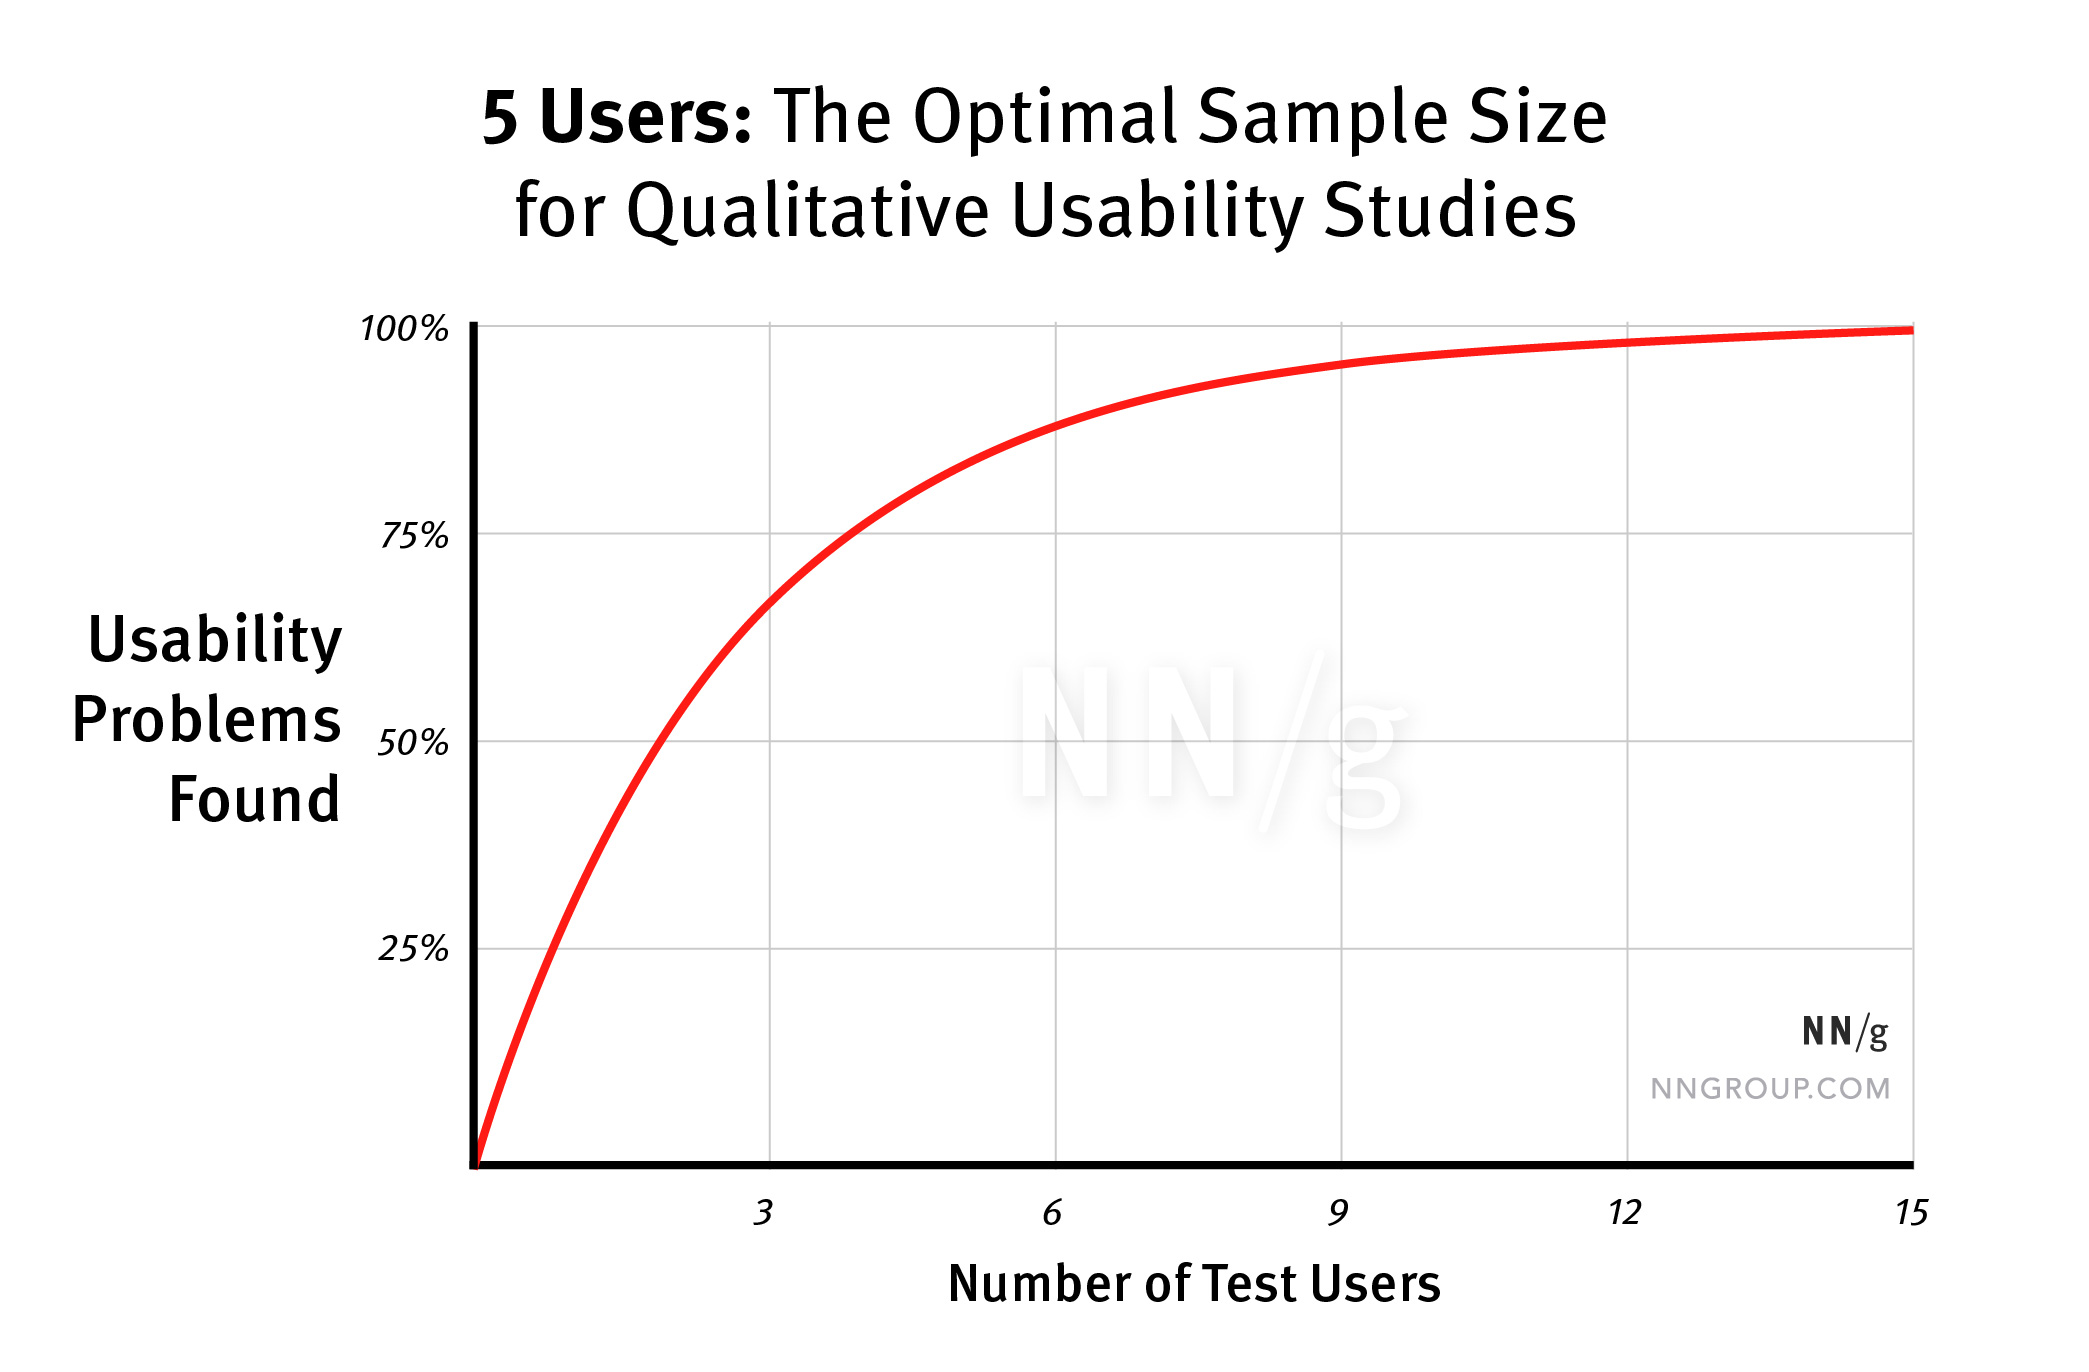
\includegraphics[width=5cm]{./figure/figure_fiveUsers.png}}
    \caption{กราฟแสดงความสัมพันธ์ของสมการ}\label{fig:model7}
\end{figure}
\par เมื่อมองจากอัตราการได้รับข้อมูล พบว่า เส้นความชันจะเริ่มต่ำลงตั้งแต่จำนวน 
3-5 คน และเริ่มหยุดนิ่ง จึงสามารถสรุปได้ว่า จำนวนผู้ใช้เพื่อการสัมภาษณ์ที่ดี
ในการค้นหาข้อมูลเชิงลึกหรือปัญหา ควรอยู่ที่ราว ๆ 5 คน
\par อย่างไรก็ตาม ทฤษฎีนี้สามารถนำไปปรับใช้เพิ่มเติมได้ เช่น หากผู้ใช้มีกลุ่มเฉพาะ
ที่ชัดเจนหลายกลุ่ม เราสามารถเปลี่ยนจำนวนการทดสอบเป็น 3-4 คนต่อกลุ่ม 
เนื่องจากข้อมูลบางอย่างอาจมีการทับซ้อนกันระหว่างกลุ่มได้ด้วย \\
\textbf{การนำไปใช้งาน} : ทางคณะผู้จัดทำ ได้นำหลักการนี้ไปปรับใช้กับ
การเลือกกลุ่มตัวอย่างและจำนวนในการสัมภาษณ์เพื่อเก็บข้อมูลเชิงคุณภาพ 
หรือการทดสอบวิธีการแก้ปัญหาที่เราออกแบบกับผู้ใช้ โดยคาดหวังว่า 
จะได้รับข้อมูลที่เห็นแนวโน้มในภาพรวมจากจำนวนในทฤษฎี 
ประหยัดเวลาที่ใช้ในการศึกษากลุ่มเป้าหมายและเน้นไปที่ประสิทธิภาพมากขึ้น
\subsection{Usability Heuristics Principles}
การออกแบบส่วนต่อประสานกับผู้ใช้ (User Interface Design) 
เป็นกระบวนการที่ให้ความสำคัญกับประสิทธิภาพในการใช้งานและประสบการณ์ของผู้ใช้ 
ซึ่งหนึ่งในเครื่องมือที่มีประสิทธิภาพในการประเมินการออกแบบนั้นคือ 
"Usability Heuristics Principles" ซึ่งถูกพัฒนาโดย Jakob Nielsen  
ในปี 1994 โดยมีเป้าหมายเพื่อช่วยนักออกแบบในการพัฒนาและปรับปรุงการออกแบบ
ส่วนต่อประสานกับผู้ใช้ให้ดีขึ้น โดย Usability Heuristics มีหลักการทั้ง 10 ข้อ ดังนี้
\begin{enumerate}
    \item \textbf{Visibility of System Status} 
    ผู้ใช้ควรทราบสถานะปัจจุบันของระบบตลอดเวลา โดยการใช้สถานะแสดงอย่างชัดเจน 
    เช่น แถบความคืบหน้า หรือสถานะการทำงาน
    \item \textbf{Match between System and the Real World} 
    การออกแบบควรสอดคล้องกับความคาดหวังและความรู้ของผู้ใช้ในโลกแห่งความเป็นจริง 
    เพื่อลดความสับสนและเพิ่มความเรียบง่ายในการใช้งาน
    \item \textbf{User Control and Freedom} 
    ผู้ใช้ควรมีอิสระในการยกเลิกหรือย้อนกลับการกระทำที่เกิดขึ้นโดยไม่ก่อให้เกิด
    ความรู้สึกกังวลหรือติดอยู่กับขั้นตอนนั้น ๆ  และต้องมีทางออกฉุกเฉินในกรณีที่ผู้ใช้
    ไม่ต้องการทำการกระทำเหล่านั้น
    \item \textbf{Consistency and Standards} 
    การออกแบบควรปฏิบัติตามมาตรฐานทีได้กำหนดไว้ ตั้งแต่การออกแบบกราฟิกไป
    จนถึงรูปแบบการใช้งาน เพื่อให้ผู้ใช้งานสามารถจดจำและใช้งานได้ง่ายด้วยการสร้าง 
    Design System เพื่อวางแนวทางในการออกแบบ
    \item \textbf{Error Prevention} 
    การออกแบบควรป้องกันข้อผิดพลาดจากการเกิดขึ้น ด้วยการมีการเตือนให้ผู้ใช้
    ตรวจสอบความถูกต้องก่อนที่จะทำอะไรบางอย่างที่สำคัญหรือร้ายแรง
    \item \textbf{Recognition rather than Recall} 
    ผู้ใช้ควรสามารถรู้จักและใช้งานส่วนต่อประสานได้อย่างเหมาะสมโดยไม่ต้องใช้ความรู้
    หรือความจำที่มากเกินไป
    \item \textbf{Flexibility and Efficiency of Use} 
    การออกแบบควรสนับสนุนการใช้งานของผู้ใช้ที่มีความสามารถในการใช้งานมากและ
    น้อยอย่างมีประสิทธิภาพ
    \item \textbf{Aesthetic and Minimalist Design} 
    การออกแบบควรใช้ข้อความและสัญลักษณ์ให้มีความชัดเจน รวมถึงสวยงามและเรียบง่าย 
    โดยไม่ทำให้ผู้ใช้งานเกิดความสับสนและไม่มากจนเกินไป
    \item \textbf{Help Users Recognize, Diagnose, and Recover from Errors} 
    การออกแบบควรช่วยให้ผู้ใช้รู้ว่าเกิดข้อผิดพลาดอะไรขึ้น และมีแนวทางสำหรับ
    การแก้ไขปัญหาให้ผู้ใช้ตามหาได้
    \item \textbf{Help and Documentation} 
    การออกแบบควรให้ความช่วยเหลือและเอกสารความช่วยเหลือให้ผู้ใช้เมื่อจำเป็น 
    แต่ก็ควรสร้างระบบที่ใช้งานได้โดยไม่ต้องพึงพาเอกสารอ้างอิงต่าง ๆ
\end{enumerate}
\par การใช้งาน 10 Usability Heuristics for User Interface Design 
เป็นเครื่องมือมีประสิทธิภาพในการปรับปรุงประสิทธิภาพการใช้งานและประสบการณ์ของ
ผู้ใช้ในเว็บไซต์และแอปพลิเคชัน โดยการปฏิบัติตามหลักการเหล่านี้ 
จะทำให้สามารถเพิ่มคุณภาพและประสิทธิภาพของส่วนต่อประสานกับผู้ใช้ให้ดียิ่งขึ้น \\
\textbf{การนำไปใช้งาน} : ทางคณะผู้จัดทำได้นำ 
Usability Heuristics Principles ไปใช้เพื่อเป็นเกณฑ์ในการวัดความใช้งานง่าย
ของเว็บแอปพลิเคชันและรับข้อเสนอแนะของผู้ใช้เพื่อนำมาปรับปรุงให้ประสบการณ์
ของผู้ใช้ในการใช้งานเว็บแอปพลิเคชันดีมากยิ่งขึ้น

\subsection{Artificial Neural Network (ANN)}
เป็นแนวคิดเพื่อนำมาใช้ในการสร้างโมเดล machine learning โดยใช้วิธีการสร้างโครงข่ายประสาทเทียม
และมีการสร้างเครื่องที่ชื่อว่า Perceptron เพื่อนำมาใช้ทดลองตั้งแต่ปี 1958

อัลกอริทึมที่ใช้ในการฝึกฝนโมเดล ANN จะประกอบด้วยพื้นฐาน ดังนี้
\begin{enumerate}
    \item \textbf{สุ่มค่าเริ่มต้นของ w และ b} 
    \item \textbf{เลือกค่า learning rate r ระหว่าง 0 และ 1} 
    \item \textbf{สำหรับจุดข้อมูล (x,y) คำนวณค่า f(x) = w*x + b} 
    \item \textbf{ปรับค่า w และ b โดยใช้สมการ w = w + r(y - f(x))x และ b = b + r(y - f(x))} 
    \item \textbf{ทำซ้ำตามจำนวนครั้งที่ต้องการหรือจนกว่าอัตราความผิดพลาดจะน้อยกว่าที่กำหนด} 
\end{enumerate}
โดยที่ w เป็นเวกเตอร์น้ำหนัก และ b เป็นค่าไบแอสที่โมเดลจะเรียนรู้ขึ้นมาระหว่างการฝึกฝน

อย่างไรก็ตาม รูปแบบนี้ยังมีข้อจำกัด เช่น ไม่สามารถทำนายความสัมพันธ์แบบ XOR ได้ ดังนั้นจึงมีการเพิ่มน้ำหนักของสมการตัดสินใจนี้ ดังนี้
\[
    y=x_{1}\oplus x_{2}=f(x)=
    \begin{cases} 
    1, & if w \cdot w + b = w_{1}x_{1} + w_{2}x_{2} + w_{3}x_{1}x_{2} + b > 0 \\
    0, & otherwise \\
    \end{cases}
\]

และต่อมายังเพิ่มขีดความสามารถให้โมเดลมีความยืดหยุ่นมากขึ้น โดยการพัฒนาขั้นต่อมานั้น เป็นการเพิ่ม layer ของ Perceptron เข้าไป โดยมีฟังก์ชันที่ไม่เป็นเชิงเส้นคั่นระหว่าง layers ดังนั้น ฟังก์ชันของแต่ละ layer คือ
\[f(x)=\sigma(w \cdot x + b)\]

โครงสร้างพื้นฐานของโมเดล Multi-layer Perceptron ประกอบไปด้วย 3 ส่วน ได้แก่ input layer, hidden layer และ output layer โดยสามารถมี hidden layer ได้หลาย layer ตามความต้องการของผู้ออกแบบโมเดล

จากสิ่งที่กล่าวมาทั้งหมดนี้ ANN ได้กลายเป็นพื้นฐานของโมเดลประเภทโครงข่ายประสาทเทียม และถูกนำไปปรับปรุงให้กลายเป็นโมเดลรูปแบบใหม่ ๆ เพื่อสร้างจุดเด่นกับงานเฉพาะด้าน เช่น การนำ output ของ layer ท้าย ๆ ป้อนกลับเข้าไปใน layer ก่อนหน้าพร้อมกับข้อมูลใหม่ (RNN) หรือ เชื่อม layer ต่าง ๆ โดยเชื่อมเฉพาะ neuron ที่อยู่ใกล้กันเท่านั้น ไม่ได้เชื่อมหมดทั้ง layer (CNN)
\textbf{การนำไปใช้งาน} : ทางคณะผู้จัดทำได้ศึกษาพื้นฐานของระบบโครงข่ายประสาทเทียมเพื่อนำมาเป็นส่วนหนึ่งของการพัฒนาโมเดลปัญญาประดิษฐ์ภายในเว็บแอปพลิเคชันของเราทุกอัน รวมถึงถูกนำมาใช้งานในการฝึกฝนโมเดลเพื่อทดสอบประสิทธิภาพและเปรียบเทียบกับโมเดลอื่น ๆ อีกด้วย


\subsection{Recurrent Neural Network (RNN)}
RNN เป็นระบบโครงข่ายประสาท (neural network) ที่จะนำ output จาก state 
ก่อนหน้ามาเป็น input ในรอบใหม่ ทำให้สามารถเข้าใจข้อมูลประเภทที่มีลำดับได้ดี จำพวก 
ข้อความ หรือข้อมูลที่เป็นลำดับเวลา (time-series) โดยมีสมการดังนี้
    \[h(t) = x(t) W_{in} + h(t-1)W\]
\par โดยสมการนี้แสดงถึงการที่ใช้ค่า Output ของ x(t) ร่วมกับ Output ของ h(t-1) 
(output ของ network ที่แล้ว) โดยมี Weight 2 ตัวปรับของ x(t) กับ h(t-1)
\par อย่างไรก็ตาม RNN จะพบข้อปัญหาบางอย่างได้ง่าย เช่น 
การใช้งานหน่วยความจำนวนปริมาณมากจากการวนรอบ หรือการแบ่งน้ำหนัก (weight) 
ที่อาจยังทำได้ไม่ดีนักหากใช้วิธีปกติ ดังนั้น จึงมีการนำ RNN 
ไปพัฒนาต่อจนเกิดเป็นรูปแบบใหม่ (variant) ที่แก้ปัญหาเดิมได้ เช่น LSTM และ GRU \\
\textbf{การนำไปใช้งาน} : ทางคณะผู้จัดทำได้ศึกษาหลักการพื้นฐานของ RNN 
เพื่อนำไปเป็นพื้นฐานของการศึกษาเนื้อหาอื่น ๆ ต่อไป เช่น LSTM และ GRU 
ซึ่งอาจนำไปใช้เปรียบเทียบประสิทธิภาพกับหลักการอื่นอีกทีหนึ่ง
\subsection{Long Short Term Memory (LSTM)}
\label{subsec:lstm}
เป็น RNN ที่นำมาพัฒนาต่อ ทำงานได้ดีขึ้นกับข้อมูลที่จำเป็นต้องมีการเรียนรู้แบบระยะยาว เพราะมีการกำหนดน้ำหนักสำหรับการลืมเอาไว้ให้สำหรับ model ด้วย ซึ่งจะช่วยลดปริมาณหน่วยความจำที่ใช้ได้ ซึ่งเป็นปัญหาที่พบได้จาก RNN ปกติ โดยภายใน LSTM จะมีตัวแปรที่สำคัญ ดังนี้
\begin{itemize}
    \item \textbf{Cell state} เป็นตัวเก็บ state ของ memory cell ใน LSTM
    \item \textbf{Gate} เป็นตัวที่ควบคุมการไหลของข้อมูล ซึ่งเป็นรูปแบบ 0/1 (อนาล็อก) ที่จะควบคุมว่าเมื่อไหร่จะทำการ อ่าน เขียน หรือ ลืม (forget) ซึ่งเหมือนกับประตูที่จะออกคำสั่งว่า เมื่อไหร่ควรเปิดให้ข้อมูลไหลเข้า ไหลออก หรือควรลบทิ้ง
\end{itemize}
โดยจากที่กล่าวไป คำสั่งที่สำคัญภายใน gate ของ LSTM จะประกอบด้วย
\begin{enumerate}
    \item \textbf{การลืม (forget)} เป็นการลืมข้อมูลเดิมเพื่อไปรับข้อมูลใหม่ 
    โดยจะตัดสินการลืมนี้ด้วย forget gate ซึ่งจะส่งสัญญาณ 0/1 ออกมา การสร้าง 
    forget gate นี้ เราจะดู input data ที่เข้ามา ประกอบกับ hidden state 
    ก่อนหน้า (ตามหลักการของ RNN) ประกอบการตัดสินใจ โดยจะใช้ 
    sigmoid function เป็นตัวตัดสิน ดังสมการ
        \[f_t = \sigma(W_{x^f}x_t + W_{h^f}h_{t-1}+b_f) \]
    \item \textbf{การเขียน (write)} ก่อนจะเกิดการเขียนข้อมูลใหม่ 
    จำเป็นต้องมีการตัดสินก่อนว่า จำเป็นต้องมีการเปลี่ยนแปลงค่าหรือไม่ 
    หากต้องมีการเปลี่ยนแปลง จะเปลี่ยนแปลงเป็นอะไร โดยการตัดสินขั้นแรก 
    จะใช้งานผ่าน input gate และใช้ sigmoid function เป็นตัวตัดสินเช่นเดิม 
    (สามารถใช้สมการเดิมได้เหมือนกับสมการการลืม)
    \par ซึ่งในกรณีต้องมีการเปลี่ยนแปลง จะใช้ Input modulation gate 
    เป็นตัวจัดการ โดยสมการก็จะเหมือนกับ input gate แต่ว่าจะใช้เป็น 
    tanh function ซึ่งค่าที่ได้นั้น เปรียบได้เป็น cell state candidate
        \[ g_t = tanh(W_{x^c}x_t + W_{h^c}h_{t-1}+b_c) \]
    \par ดังนั้น วิธีการคำนวณค่าใหม่สำหรับการเปลี่ยนแปลง จะเป็นไปดังสมการ
        \[c_t = f_t \odot c_{t-1}+i_t \odot g_t \]
    \par หาก gate ใด ๆ ส่งสัญญาณเป็น 0 ก็จะส่งผลให้ไม่นำค่าต่าง ๆ มาใช้ เช่น 
    หากค่าจาก f (forget gate) เป็น 0 ค่าของ c ก็จะถูกลืมและไม่นำมาพิจารณา 
    แต่หากเป็น 1 แสดงว่ามีความต้องการจะเปลี่ยนแปลงข้อมูล ซึ่งจะตัดสินว่าควรใช้ค่าใหม่
    เป็นค่าใดจาก input modulation gate หากเป็น 1 ก็จะนำ g ไปใช้งานนั่นเอง
    \item \textbf{การอ่าน (read)} เนื่องจากค่า output ที่ได้รับมาในขั้นตอน
    ก่อนหน้า เป็น output ณ เวลาต่าง ๆ ใน hidden state นั้น 
    เราจึงสามารถคำนวณค่า ณ เวลานั้นกลับมาได้ด้วยสูตรเดิมเหมือนในขั้นตอนก่อนหน้า 
    เพียงแต่ในขั้นตอนการอ่านนั้น จะมีการใช้งาน output gate มาช่วยติดสินว่า
    ควรอนุญาตให้อ่านข้อมูล ณ ตอนนั้นหรือไม่ โดยสูตรคำนวณจะเหมือนกับ 
    forget gate และ input gate อย่างที่เคยกล่าวไป นั่นคือ ใช้ 
    sigmoid function กับค่า hidden state ตัวก่อนหน้า กับ input data 
    ที่เข้ามาในตอนนั้น
        \[ o_t = \sigma (W_{x^o}x_t+W_{h^o}h_{t-1}+b_o) \]
    \par จากค่าของ open gate ในสูตรดังกล่าว จะเขียนสมการในการอนุญาตให้อ่าน
    ข้อมูลได้ดังนี้
        \[ h_t = o_t \odot tanh(c_t) \]
\end{enumerate}
\textbf{การนำไปใช้งาน} : เป็นหนึ่งในทางเลือกที่ทางคณะผู้จัดทำได้ศึกษา
เพื่อนำความรู้ไปพิจารณาใช้งานกับวิธีการแก้ปัญหาที่ทางคณะผู้จัดทำออกแบบ ซึ่ง LSTM 
สามารถนำไปใช้งานและตอบโจทย์การทำ Text-based Generative AI ได้ 
อย่างไรก็ตาม คณะผู้จัดทำยังมีข้อจำกัดเรื่องของปริมาณข้อมูลที่สามารถนำมาใช้ 
และประสิทธิภาพที่เมื่อเทียบกับ model ประเภทอื่นในปัจจุบัน อาจด้อยกว่าเล็กน้อย 
จึงอาจเป็นตัวเลือกรอง แต่ก็ถือว่าเป็นหนึ่งในตัวเลือกที่น่าสนใจไม่น้อย

\subsection{SQL และ NoSQL}
sql หรือ Structured query Language เป็นภาษาโปรแกรมมิ่งชนิดหนึ่ง 
ที่ใช้ในการสื่อสารกับ ฐานข้อมูลชนิดที่มีความสัมพันธ์ หรือที่เรียกว่า RDBMS 
(Relational Database Management System) ซึ่งมีวิธีการเก็บข้อมูลในรูปแบบ
ของตาราง (table) โดยภายในหนึ่งตารางจะประกอบด้วย
\begin{enumerate}
    \item \textbf{Row (แถว หรือ แนวนอน)} เรียกอีกชื่อว่า Tuple คือ 
    ตัวเนื้อข้อมูล
    \item \textbf{Column (สดมภ์ หรือ แนวตั้ง)} เรียกอีกชื่อว่า Attribute 
    คือ การระบุชนิดของข้อมูลนั้น ๆ เช่น ที่อยู่, วัน เดือน ปีเกิด, ตัวเลข
\end{enumerate}
\par โดยแต่ละตารางจะเชื่อมความสัมพันธ์กันด้วยข้อกำหนดที่เรียกว่า key 
ซึ่งมีสองรูปแบบคือ
\begin{enumerate}
    \item \textbf{Primary Key} หมายถึง การกำหนดรูปแบบของ column 
    ที่จะไม่เกิดการซ้ำกันได้ และไม่มีทางเกิดข้อมูลว่าง
    \item \textbf{Foreign Key} หมายถึง ต้องมีการอ้างอิงถึงข้อมูลประเภทเดียวกัน
    จากตารางที่มี Primary Key อยู่ภายใน
\end{enumerate}
\par NoSQL หรือ Non-relational database เป็นฐานข้อมูลที่มีความสัมพันธ์กัน
ชัดเจนแบบ เหมาะสำหรับการใช้งานกับ Real-time Web Application 
โดยประเภทของ NoSQL จะแบ่งออกเป็น 4 แบบหลัก ๆ ได้แก่
\begin{enumerate}
    \item \textbf{Document} ข้อมูลจะเก็บเป็นลำดับชั้นในรูปแบบ 
    Semi-structure data เช่น JSON
    \item \textbf{Key-value} ข้อมูลจะเก็บในรูปแบบแถว (record) ที่ประกอบด้วย 
    key และ value ที่เชื่อมกันแบบหนึ่งต่อหนึ่ง เข้าถึงข้อมูลได้เร็ว
    \item \textbf{Graph} ข้อมูลจะเก็บอยู่ในรูปแบบกราฟแผนภูมิ มี Node และ Edge 
    ที่เชื่อมต่อกัน ทำให้ไม่ต้องนำข้อมูลมาเชื่อม (join) เหมือนกับวิธีการของ RDBMS
    \item \textbf{Wide-Column} บันทึกข้อมูลในรูปแบบ table (row/column) 
    แต่จะต่างจาก RDBMS ตรงที่แต่ละ row จะไม่กำหนดหรือบังคับประเภท column
\end{enumerate}
\textbf{การนำไปใช้งาน} : ทางคณะผู้จัดทำได้พิจารณาจากรูปแบบของข้อมูล
ที่ต้องเก็บเป็นหลัก ความสะดวกของบริการที่สามารถนำมาใช้งาน และพิจารณา
ในความเหมาะสมของการพัฒนาแล้ว โดยเพ่งเล็งว่า จะมีการนำฐานข้อมูลในรูปแบบ NoSQL 
ประเภท document มาใช้งานเป็นหลัก โดยมีบริการที่น่าสนใจและเอื้อมถึงได้ง่าย 
เช่น MongoDB
\section{อัลกอริทึมในการแปลผลภาษา}
\subsection{Term Frequency Inverse Document Frequency (TF-IDF)}
\label{subsec:tf-idf}
เป็นอัลกอริทึมที่ผสมผสานกันระหว่าง Term-Frequency (TF) และ Inverse Document Frequency (IDF) ซึ่งเป็น
เทคนิคพื้นฐานเทคนิคหนึ่งที่ใช้ในการวิเคราะห์ค้นหาคำสำคัญของข้อมูลในลักษณะของข้อความ \cite{tf-idf}
\begin{itemize}
    \item \textbf{Term-Frequency (TF)} โดยจะคำนวณเป็นอัตราส่วนของจำนวนคำนั้น ๆ ต่อจำนวนคำทั้งหมดในเอกสาร
    เพื่อหาว่าคำนั้นมีความถี่เท่าไหร่
    \begin{figure}[!h]\centering
        \setlength{\fboxrule}{0.2mm} % can define this in the preamble
        \setlength{\fboxsep}{1cm}
        \fbox{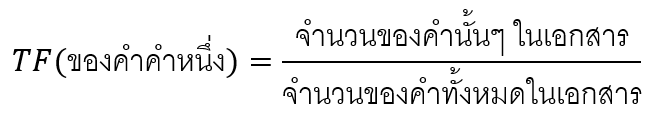
\includegraphics[width=5cm]{./figure/figure_tf.png}}
        \caption{สมการการคำนวณ Term-Frequency (TF)}\label{fig:model4}
    \end{figure}
    \item \textbf{Inverse Document Frequency (IDF)} โดยจะคำนวณความสำคัญของแต่ละคำโดยคำที่พบได้บ่อยจะมีค่า IDF ที่ต่ำ
    ซึ่งบ่งบอกว่าคำเหล่านั้นไม่สามารถดึงเอาจุดเด่นของเอกสารออกมาได้ดี
    \begin{figure}[!h]\centering
        \setlength{\fboxrule}{0.2mm} % can define this in the preamble
        \setlength{\fboxsep}{1cm}
        \fbox{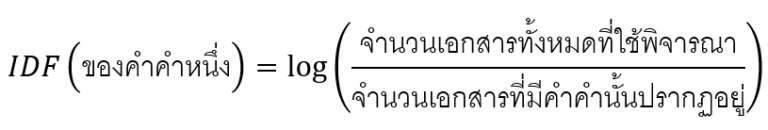
\includegraphics[width=5cm]{./figure/figure_idf.png}}
        \caption{สมการการคำนวณ Inverse Document Frequency (IDF)}\label{fig:model5}
    \end{figure}
    \item \textbf{คำนวณค่า TF-IDF} โดยเราจะนำ TF กับ IDF มาคำนวณและถ้าหากคำไหนที่มาค่า TF-IDF ที่สูง จะถูกมองว่าเป็นคำที่มีความสำคัญ
    สูง (กล่าวถึงบ่อย แต่ก็ไม่ได้ปรากฏอยู่หลายเอกสารเกินไป) และมีแนมโน้มจะเป็นใจความสำคัญของเอกสาร
    \[TFIDF = TF * IDF\]
\end{itemize}
\section{อัลกอริทึมในการแยกประเภทเรซูเม}
\subsection{อัลกอริทึม I K-Nearest Neighbors (KNN)}

% Can define this in the preamble..
เป็นอัลกอริทึมสำหรับการจัดกลุ่มข้อมูล (Classfication) ซึ่งอยู่ในกลุ่มของการเรียนรู้แบบมีผู้สอน (Supervised Learning)
หลักการทำงาน คือการจัดกลุ่มโดยอิงถึงความใกล้เคียงของข้อมูล เพื่อคาดเดาหรือจำแนกประเภทข้อมูลใหม่ \cite{kNeighbor} โดยหลักการทำงานสามารถสรุปได้ดังนี้
\begin{enumerate}
    \item  \textbf{เลือกค่า K} : กำหนดค่า K ที่ต้องการ ซึ่งเป็นจำนวนของข้อมูลที่ใกล้ที่สุดที่จะใช้ในการตัดสินใจ
    \item  \textbf{คำนวณระยะทาง} : ใช้ระยะทางยูคลิเดียน (Euclidean distance) เพื่อคำนวณหาความคล้ายคลึงระหว่างข้อมูล
    \item  \textbf{หาข้อมูลที่ใกล้ที่สุด} : หลังจากคำนวณระยะทางระหว่างข้อมูลทดสอบกับข้อมูลในชุดข้อมูลการฝึกฝน เราจะเลือกข้อมูล K รายการที่มีระยะทางน้อยที่สุด
    \item  \textbf{คำนวณผลโหวต} : เมื่อเราได้ข้อมูล K รายการที่ใกล้ที่สุดแล้ว เราจะนับจำนวนรายการในแต่ละกลุ่มหรือประเภทข้อมูล 
    และกำหนดกลุ่มหรือประเภทข้อมูลของข้อมูลทดสอบตามจำนวนที่มากที่สุดใน K รายการนั้น
    \item  \textbf{ทำนายผลลัพธ์} : สุดท้ายเราก็จะได้กลุ่มข้อมูลที่ถูกแบ่งออกมาพร้อมใช้ในการทำนายต่อไป
\end{enumerate}

\begin{figure}[!h]\centering
    \setlength{\fboxrule}{0.2mm} % can define this in the preamble
    \setlength{\fboxsep}{1cm}
    \fbox{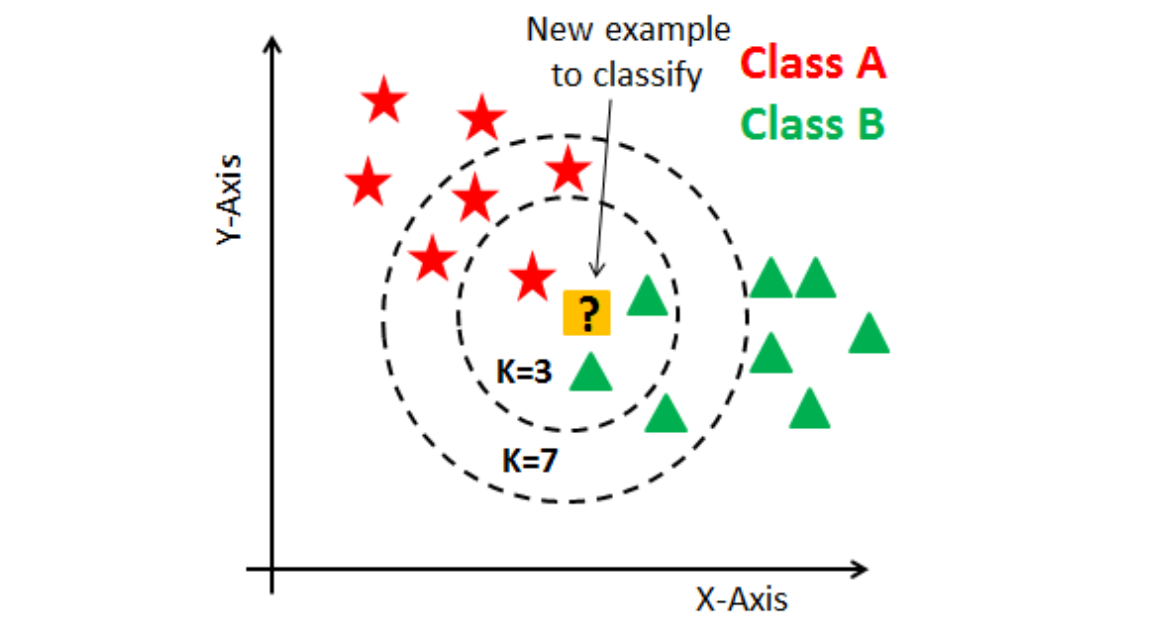
\includegraphics[width=5cm]{./figure/figure_knn.png}}
    \caption{ลักษณะการทำงานของ K-Nearest Neighbors}\label{fig:model2}
\end{figure}

\subsection{อัลกอริทึม II Naive Bayes Classifier}
Naive Bayes Classification เป็นหนึ่งใน Classification Model ใช้ในการแบ่งกลุ่มหรือหาเหตุการณ์ที่จะเกิดขึ้นโดยการอิงทฤษฎีความน่าจะเป็นของ 
Bayes หรือ Bayesian 
\par ซึ่งจะคำนวณว่าจะเกิดเหตุการณ์นั้นหรือไม่โดยจะเพิ่มโอกาสในการเกิดเหตุการณ์เข้าไปด้วย 
โดยมักจะใช้ในการวิเคราะห์ข้อมูลที่มีความต่อเนื่องของเหตุการณ์ (Dependent Event) เช่น 
โอกาสในการเกิดโรคในกลุ่มประชากรที่เราสนใจ \cite{naiveBayes-1,naiveBayes-2} ซึ่งจำเป็นจะต้องอาศัยการคำนวณผ่านสูตรดังนี้ และกำหนดให้

\begin{figure}[!h]\centering
    \setlength{\fboxrule}{0.2mm} % can define this in the preamble
    \setlength{\fboxsep}{1cm}
    \fbox{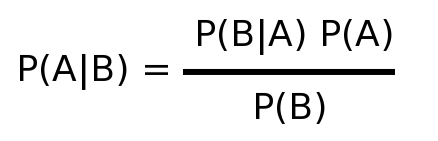
\includegraphics[width=5cm]{./figure/figure_nb.png}}
    \caption{สมการความน่าจะเป็นของ Bayes หรือ Bayesian}\label{fig:model3}
\end{figure}

\par P(A|B) คือความน่าจะเป็นในการเกิดเหตุการณ์ A โดยมี B เป็น Condition
\par P(B|A) คือความน่าจะเป็นในการเกิดเหตุการณ์ B โดยมี A เป็น Condition
\par P(A) คือโอกาสในการเกิดเหตุการณ์ A จากเหตุการณ์ทั้งหมด
\par P(B) คือโอกาสในการเกิดเหตุการณ์ B จากเหตุการณ์ทั้งหมด
\section{ภาษาคอมพิวเตอร์ และเทคโนโลยี}
\subsection{เครื่องมือในการทำโครงงาน}
\subsubsection{Figma}
\label{subsec:Figma}
เครื่องมือที่ใช้ในการออกแบบส่วนต่อประสานผู้ใช้ (User Interface) รวมถึงระดมสมอง (Brain Storm) 
และใช้สำหรับให้นักออกแบบสื่อสารกับผู้อื่นให้เข้าใจได้ง่ายและเห็นภาพมากยิ่งขึ้น 
เช่น การทำ User Persona, User Journey, User Flow, Site Map รวมถึงการทำ 
Prototype เพื่อนำมาใช้ในการทดสอบการใช้งานของผู้ใช้ (Usability Test) 
และยังสามารถออกแบบดีไซน์ของเว็บไซต์ (Design System) 
เพื่อให้นักพัฒนาสามารถนำสไตล์ไปใช้พัฒนาเว็บFไซต์ได้ง่ายและเป็นระเบียบมากยิ่งขึ้น
\subsubsection{Jira}
เครื่องมือที่ช่วยในการพัฒนาซอฟต์แวร์ทางอ้อม มีส่วนช่วยในการติดตามและจัดการงานต่าง ๆ 
ได้ถึงระดับย่อย เหมาะสมกับการทำงานในรูปแบบ Agile อีกทั้งยังสามารถผูกกับบริการต่าง ๆ 
ภายนอกได้ ทำให้การติดตามงานสะดวกยิ่งขึ้นไปอีก
\subsection{ภาษาโปรแกรมที่ใช้}
\subsubsection{Typescript}
ภาษาที่พัฒนาต่อยอดมาจาก Javascript เพื่อปรับปรุงจุดด้อยต่าง ๆ เช่น การจัดการ 
interface และประเภทของตัวแปร การเขียนโค้ดที่สนับสนุนรูปแบบ OOP ที่ดีกว่า 
การตรวจจับข้อผิดพลาดและการรับมือที่ดีกว่า โดยทางเราจะนำมาใช้งานกับ framework 
ต่าง ๆ ที่กล่าวไปข้างต้น เพื่อให้การทำงานมีประสิทธิภาพสูงสุด
\subsubsection{Python}
ภาษาโปรแกรมที่ถูดจัดอยู่ในประเภทระดับสูง ซึ่งถูกนำมาใช้อย่างแพร่หลายในปัจจุบัน 
มีลักษณะไวยากรณ์ไม่ซับซ้อน สามารถใช้พัฒนาเว็บแอปพลิเคชัน 
รวมถึงนำไปประยุกต์พัฒนาปัญญาประดิษฐ์ได้หลายประเภท 
มีไลบรารี่จำนวนมาก อีกทั้งยังชุมชนใหญ่ ซึ่งในที่นี้ เราจะนำมาใช้สำหรับการพัฒนาปัญญาประดิษฐ์ของเรา
\subsection{เทคโนโลยีจัดการระบบหน้าบ้าน (Front-End)}
\subsubsection{NextJS}
React framework ซึ่งสามารถใช้สร้าง full-stack web applications ได้ 
แต่ทางเราจะมุ่งเน้นไปที่การนำมาใช้พัฒนาส่วน frontend โดย NextJS 
จะมีความสามารถในการเขียนส่วนปฏิสัมพันธ์กับผู้ใช้ในเชิง components 
เหมือนกับ React และมีส่วนเสริมต่าง ๆ เพื่อให้การทำงานของเราเป็นไปอย่าง
มีประสิทธิภาพมากขึ้น เช่น routing, caching , optimizing, configuration 
ต่าง ๆ
\subsection{เทคโนโลยีจัดการระบบหลังบ้าน (Back-End)}
\subsubsection{NestJS}
Framework ที่ใช้สำหรับพัฒนาระบบ backend ซึ่งเขียนด้วยภาษา TypeScript 
โดยมีพื้นหลังของการพัฒนา framework มาจาก Express และ Fastify 
โดยมุ่งเน้นให้นักพัฒนาสามารถพัฒนาระบบ backend ได้อย่างรวดเร็ว 
และสนับสนุนหลักการทำงานต่าง ๆ ที่นักพัฒนานิยมใช้งาน 
โดยทางเราเองก็จะใช้ความสามารถในส่วนนี้เพื่อนำมาใช้พัฒนาเช่นกัน อาทิ REST API 
และ MVC structure
\subsection{บริการคลาวด์ (Cloud Service)}
\subsubsection{Google Cloud Platform (GCP)}
บริการในรูปแบบ cloud ของทาง Google ซึ่งประกอบด้วยบริการหลากหลายรูปแบบ 
โดยทางเรามุ่งเน้นที่จะใช้งานบริการส่วนของการหลัก ๆ ดังนี้
\begin{itemize}
    \item \textbf{Cloud Run} : บริการสำหรับการนำ container ที่มีมารันบน cloud โดยเราจะนำบริการนี้มา host ทั้งในส่วนของหน้าบ้านและหลังบ้านของเว็บแอป
    \item \textbf{Cloud Build} : บริการสำหรับนำไฟล์โปรเจ็กต์มา build ให้อยู่ในรูปแบบ container โดยเราจะนำมาใช้คู่กับ docker เพื่อนำโปรเจ็กส่งสู่ Cloud Run
    \item \textbf{Cloud Storage} : บริการสำหรับเก็บไฟล์มีเดียต่าง ๆ เช่น รูปภาพ เสียง วิดีโอ เพื่อนำมาเก็บข้อมูลของผู้ใช้ที่เป็นมีเดีย
    \item \textbf{Artifact Registry} : บริการสำหรับเก็บไฟล์ container ต่าง ๆ ที่มีทั้งหมด โดยนำมาใช้คู่กับ Cloud Build เพื่อเก็บ container ที่ผ่านการ build เสร็จแล้ว
\end{itemize}

\subsection{ระบบฐานข้อมูล}
\subsubsection{MongoDB}
Open-source database ประเภท NoSQL ที่มีโครงสร้างแบบ document 
ซึ่งได้รับความนิยมอย่างสูงเนื่องจากยืดหยุ่นและปรับขนาดได้ง่าย 
อีกทั้งยังรอบภาษาที่หลากหลายทั้ง Javascript, Python, Java และอื่น ๆ 
โดยทางเราเลือกใช้งาน MongoDB เพราะมีเงื่อนไขที่ยืดหยุ่นเหมาะกับการทำงานของเรา 
เช่น ไม่จำกัดจำนวนคำขอ API ต่อวัน และมีพื้นที่จัดเก็บที่พอเหมาะอยู่ที่ 512 GB 
ในระดับการใช้งานฟรี
\subsection{เครื่องมือช่วยเหลือการพัฒนา (CI/CD Management)}
\subsubsection{Docker}
เครื่องมือที่สามารถช่วยจำลองสภาพแวดล้อมของเซิร์ฟเวอร์ด้วยหลักการ container 
และ images ทำให้ขจัดปัญหาละเอียดอ่อน เช่น ปัญหาสภาพแวดล้อมในแต่ละเครื่องไม่เหมือนกันส่งผลให้รันไม่ได้ โดยเราจะนำ docker มาใช้เป็นส่วนช่วยเหลือในการนำบริการไปปล่อยสู่สาธารณะผ่าน Google Cloud
\subsubsection{Github}
ระบบควบคุมเวอร์ชัน สามารถสร้างจุด commit เพื่อเสมือนเป็นจุดบันทึกเวอร์ชันหนึ่ง 
และสามารถนำไปเก็บบนที่เก็บรวม (repository) เพื่อควบคุมเวอร์ชันของไฟล์งาน
กับบุคคลภายในทีมได้ โดยทางเราจะนำมาใช้เพื่อควบคุมเวอร์ชันของซอฟต์แวร์โครงงาน 
เพื่อให้ทำงานได้อย่างลื่นไหล เช่น การแยกสาขาของงานตามฟีเจอร์ 
การติดตามเวอร์ชันของโค้ดเพื่อค้นหาจุดกำเนิดของข้อผิดพลาดอีกทั้งยังระบุบุคคล
ผู้รับผิดชอบการทำงานส่วนนั้นได้อีกด้วย
\section{การศึกษาข้อมูลผลิตภัณฑ์ที่ใกล้เคียง}
\subsection{หนังสือหลักสูตรวิศวกรรมศาสตร์บัณฑิต สาขาวิศวกรรมคอมพิวเตอร์ มจธ.}
เป็นหนังสือที่บอกถึงรายละเอียดของแต่ละรายวิชาที่นักศึกษาวิศวกรรมคอมพิวเตอร์ได้เรียนในหลักสูตรตั้งแต่ปี 1 ถึงปี 4
โดยจะแสดงออกมาเป็นผลลัพธ์การเรียนรู้และทักษะที่ได้จากการเรียนในวิชาต่าง ๆ แต่จะไม่ได้บอกถึงอาชีพสามารถนำไปต่อยอดจากรายวิชาได้
\par ซึ่งทางคณะผู้จัดจะนำข้อมูลรายวิชาในแต่ละปีการศึกษามาศึกษามาแบ่งว่า แต่ละรายวิชาสามารถนำไปต่อยอดทางใดได้บ้าง 
เพื่อมาวางแผนเส้นทางการลงวิชาเลือกที่สัมพันธ์กับระดับการศึกษาและความสนใจของผู้ใช้งานแต่ละคน

\subsection{LinkedIn}
LinkedIn เป็นเว็บแอปพลิเคชันชุมชนในสายอาชีพต่าง ๆ ที่ช่วยให้ผู้ใช้สร้างโปรไฟล์อาชีพของตนเองและเชื่อมโยงกับคนที่ใกล้เคียงในสายอาชีพ 
เว็บไซต์นี้จะช่วยให้ผู้ใช้สามารถสร้างเครือข่ายในสายอาชีพของตน แบ่งปันข้อมูลเกี่ยวกับประสบการณ์การทำงาน ประวัติการศึกษา ทักษะ ความถนัด 
รวมถึงเผยแพร่เนื้อหาที่เกี่ยวข้องกับสาขาอาชีพของพวกเขาในรูปแบบข่าวสาร ทำให้เชื่อมโยงและแลกเปลี่ยนข้อมูลกับผู้ใช้อื่น ๆ ในวงการได้ตลอดเวลา \\
โดยที่เว็บไซต์มีฟังก์ชันหลายอย่าง ประกอบด้วย :
\begin{itemize}
    \item \textbf{โปรไฟล์ผู้ใช้} : ผู้ใช้สามารถสร้างโปรไฟล์ส่วนตัวที่แสดงประสบการณ์การทำงาน การศึกษา ทักษะ และข้อมูลอื่นๆ เพื่อให้ผู้ใช้อื่นสามารถทราบรายละเอียดเบื้องต้นของพวกเขาได้
    \item \textbf{การเชื่อมโยง} : ผู้ใช้สามารถเชื่อมโยงกับคนอื่นในสายอาชีพ ทำให้สร้างเป็นเครือข่ายในสายอาชีพที่แข็งแกร่งขึ้น และเป็นโอกาสที่ดีให้กับผู้ใช้งานได้
    \item \textbf{โพสต์และเนื้อหา} : ผู้ใช้สามารถโพสต์เนื้อหาเกี่ยวกับวงการอาชีพ เช่น บทความ ข่าวสาร และความคิดเห็น ซึ่งช่วยในการแบ่งปันความรู้และประสบการณ์
    \item \textbf{ค้นหางาน} : ผู้ใช้สามารถค้นหางานและสมัครงานได้โดยตรงผ่านแพลตฟอร์ม และผู้ประกาศงานก็สามารถค้นหาผู้สมัครที่เหมาะสมกับตำแหน่งงานที่ว่างอยู่ของตนเองได้โดยง่าย
    \item \textbf{กลุ่มองค์กร} : บริษัทและองค์กรสามารถสร้างหรือเข้าร่วมกลุ่มบน LinkedIn เพื่อแบ่งปันข้อมูลและความรู้ในหมวดหมู่ที่เกี่ยวข้องได้ภายในกลุ่มที่กำหนดเองได้
    \item \textbf{การแสดงความสนใจ} : ผู้ใช้สามารถกดถูกใจ แสดงความคิดเห็น หรือแชร์เนื้อหาของผู้อื่น เพื่อแสดงความรับรู้ สนใจ หรือช่วยในการประกาศข่าวสารที่ดี
\end{itemize}
\par ซึ่งถือว่าเป็นเว็บแอปพลิเคชันที่เกี่ยวข้องกับการหางานที่มีความสามารถที่สูง และเน้นไปที่การสร้างคอมมูนิตี้สำหรับการทำงาน เนื่องด้วยคุณสมบัติที่หลากหลายนี้ 
ทำให้มีผู้ใช้งานเป็นจำนวนมาก ซึ่งทางคณะผู้จัดทำจะนำระบบชุมชนที่สามารถแนะนำงานกับกิจกรรม และระบบจัดเก็บเรซูเมมาต่อยอดกับโครงงานของเราให้ดียิ่งขึ้น

\subsection{JobDB}
เป็นเว็บแอปพลิเคชันที่รวบรวมตำแหน่งงานต่าง ๆ ในประเทศไทยที่กำลังเปิดรับอยู่ ที่จัดทำขึ้นมาสำหรับผู้คนที่กำลังมองหางาน \\
โดยที่เว็บไซต์มีฟังก์ชันหลายอย่าง ประกอบด้วย :
\begin{itemize}
    \item ระบบค้นหาอาชีพที่ต้องการ
    \item โพสต์ที่จะมีรายละเอียดงานที่เปิดรับ
    \item ระบบสมัครงาน
    \item คำแนะนำสำหรับการจัดทำเอกสารการสมัครงาน
    \item การแจ้งเตือนสำหรับตำแหน่งงานที่ผู้ใช้งานสนใจ
\end{itemize}
\par ซึ่งเป็นเว็บแอปพลิเคชันรวบรวมตำแหน่งงานที่เน้นกลุ่มเป้าหมายเป็นผู้ที่กำลังหางานในประเทศไทย โดยรวมมีระบบที่คอยอำนวยความสะดวกในการค้นหางานที่ผู้ใช้งานสนใจ 
และยังมีฟังก์ชันที่น่าสนใจเป็นอย่างมากกับ ระบบคำแนะนำสำหรับการจัดทำเอกสารการสมัครงาน ซึ่งทางผู้จัดทำโครงงานจะนำฟังก์ชันนี้มาต่อยอดกับโครงงานต่อไป

\subsection{Padlet}
เป็นเว็บแอปพลิเคชันที่ให้บริการบอร์ดข้อความ ที่ผู้ใช้งานสามารถเพิ่มข้อมูลต่าง ๆ ได้ ซึ่งสามารถนำมาประยุกต์ใช้ได้ในหลาย ๆ วัตถุประสงค์ เช่น 
การนำมาใช้รีวิวรายวิชาเรียนภายในกลุ่มที่กำหนด \\
โดยที่เว็บไซต์มีฟังก์ชันหลายอย่าง ประกอบด้วย :
\begin{itemize}
    \item \textbf{ระบบสร้างหน้า padlet หรือการหน้ากระดานใหม่} : โดยมีให้เลือกรูปแบบของกระดานมากมาย เช่น รูปแบบ wall, canvas, stream, Grid และอื่น ๆ 
    ที่เหมาะสมกับจุดประสงค์ที่ต้องการ
    \item \textbf{ระบบเข้าร่วมและแบ่งปัน padlet} : ทำให้สามารถเข้าไปแก้ไขหรือดูหน้า padlet ของผู้อื่นได้
    \item \textbf{ระบบแกลเลอรี} : รวมคลังหน้า padlet ให้กับผู้ใช้
    \item \textbf{ระบบเครือข่าย} : สามารถเชื่อมโยงผู้ใช้งานเว็บไซต์ Padlet เข้าด้วยกันเพื่อเสริมฟังก์ชันอื่น ๆ ได้
    \item \textbf{ระบบการทำสื่อนำเสนอ} : โดยที่จะรวบรวม padlet ต่าง ๆ มาทำเป็นสไลด์ และยังมี QR-Code ที่สามารถเข้ามาดูสไลด์ได้อีกด้วย
    \item \textbf{ระบบแจ้งเตือน} : ที่สามารถเลือกติดตาม Padlet ที่ตนเองสนใจได้
    \item \textbf{ระบบเชื่อมต่อบริการภายนอก} : ที่รวบรวมบริการไว้มากมาย เช่น ข้อมูลที่ผู้ใช้งานฝากไฟล์ออนไลน์ไว้ แม้กระทั่งระบบปัญญาประดิษฐ์ที่สามารถเพิ่มรูปภาพตามความต้องการของผู้ใช้ 
    และบริการอื่น ๆ ที่เชื่อมต่อจากภายนอก โดยมีจุดแข็งตรงที่เว็บไซต์มีบริการภายนอกเหล่านี้จำนวนมาก
    
\end{itemize}
\par ทางคณะผู้จัดทำเล็งเห็นว่ามีนักศึกษาวิศวกรรมอคมพิวเตอร์หลายคน ที่จะมาอ่านรีวิวรายวิชาก่อนที่จะเลือกลงในวิชาเลือกของตนเอง 
แต่ก็ยังมีข้อเสียที่ข้อมูลอาจจะไม่ได้อัพเดทมากเท่าที่ควร และไม่ได้จัดรูปแบบให้สามารถอ่านได้ง่าย ทางคณะผู้จัดทำจึงอยากจะนำข้อดีของบอร์ดรีวิวรายวิชาใน Padlet 
มาปรับปรุงให้ทันสมัย และอ่านได้ง่ายยิ่งขึ้น เพื่อลดข้อเสียของการใช้งาน

\subsection{JobThai}
เป็นเว็บแอปพลิเคชันสมัครงานที่มีกลุ่มเป้าหมายเป็นคนที่กำลังมองหางานในประเทศไทย ครอบคลุมหลากหลายอาชีพ \\
โดยที่เว็บไซต์มีฟังก์ชันหลายอย่าง ประกอบด้วย :
\begin{itemize}
    \item \textbf{ระบบสมัครสมาชิก} : โดยมีทั้งฝั่งของผู้ที่กำลังหางาน และผู้ที่กำลังต้องการลูกจ้าง ซึ่งแต่ละฝ่ายก็จะมีฟังก์ชันที่รองรับ เช่น ผู้ที่กำลังหางานก็จะสามารถฝากประวัติได้
    \item \textbf{ระบบค้นหางาน} : โดยสามารถคัดกรองได้ด้วยอาชีพที่ต้องการ สถานที่ทำงาน บริษัทที่เปิดรับ ประเภทของธุรกิจ รวมไปถึงเงินเดือนอีกด้วย
    \item \textbf{โพสต์} : ที่จะมีรายละเอียดงานที่เปิดรับ
\end{itemize}
\par ซึ่งเว็บแอปพลิเคชันนี้จะเน้นไปที่ผู้ใช้งานที่อยู่ในประเทศไทย และยังมีฟังก์ชันเลือกสถานที่ทำงานที่อยู่ใกล้กับสถานีรถไฟฟ้า นิคมอุตสาหกรรม หรือแม้กระทั่งใกล้กับรถเมล์ 
ซึ่งถือว่าทำมาเพื่อตอบสนองกับความต้องการของผู้ใช้งานในกรุงเทพที่ดีมาก ๆ เพราะการเดินทางก็ถือเป็นหนึ่งในปัจจัยสำคัญในการเลือกงานในปัจจุบัน

\subsection{Workday}
เป็นเว็บแอปพลิเคชันที่มุ่งเน้นไปในการจัดการทรัพยากรบุคคล โดยที่ถูกออกแบบมาเพื่อรองรับการทำงานสำหรับองค์กรขนาดกลาง จนถึงองค์กรขนาดใหญ่ \\
โดยที่เว็บไซต์มีฟังก์ชันหลายอย่าง ประกอบด้วย :
\begin{itemize}
    \item \textbf{การจัดการข้อมูลพนักงาน} : รวมถึงการจัดการการสร้าง แก้ไข และยุติข้อมูลการทำงานของพนักงาน เช่น ข้อมูลส่วนตัว การจ้างงาน การเลื่อนตำแหน่ง การลางาน เป็นต้น 
    \item \textbf{การจัดการงบประมาณ} : การคำนวณเงินเดือน การจ่ายเงินเดือน และการจัดการสวัสดิการสำหรับพนักงาน เช่น ประกันสุขภาพ กองทุนสำรองเลี้ยงชีพ เป็นต้น
    \item \textbf{การวางแผนแบบครบวงจร} : ตั้งแต่ขั้นตอนการรับสมัครงาน การบรรจุงาน การพัฒนาพนักงาน และการเลื่อนขั้น
\end{itemize}
\par ซึ่งเว็บแอปพลิเคชันนี้จะเน้นไปที่การให้บริการเกี่ยวกับการดูแลข้อมูลของพนักงาน ที่มีระบบที่น่าสนใจอย่างการวางแผนพัฒนาพนักงาน 
รวมถึงการเลื่อนขั้น ที่ทางคณะผู้จัดทำจะนำมันมาพัฒนาต่อยอดกับการพัฒนาผู้ใช้งานที่เป็นนักศึกษาวิศวกรรมคอมพิวเตอร์ต่อไป

\subsection{Camphub}
เป็นเว็บแอปพลิเคชันที่รวบรวมค่ายต่าง ๆ ในประเทศไทยที่กำลังเปิดรับสมัครอยู่ ที่จัดทำขึ้นมาสำหรับเด็กประถมจนกระทั่งรวมไปถึงบุคคลทั่วไป \\
โดยที่เว็บไซต์มีฟังก์ชันหลายอย่าง ประกอบด้วย :
\begin{itemize}
    \item การประชาสัมพันธ์ค่ายของตนเอง โดยที่ไม่ต้องเสียค่าใช้จ่าย
    \item การแบ่งประเภทของค่ายหรือมหาวิทยาลัยที่จัด เพื่อง่ายต่อการค้นหา
    \item รายละเอียดของค่าย เช่น รูปแบบกิจกรรม, วันที่จัดกิจกรรม, จำนวนที่รับ เป็นต้น
    \item การสมัครค่ายที่ตนเองสนใจ
    \item บทความต่าง ๆ ที่น่าสนใจ
\end{itemize}
\par ซึ่งเว็บแอปพลิเคชันนี้จะเน้นไปที่การรวบรวมข่าวสารกิจกรรมที่เกิดขึ้น ไม่ว่าจะเป็นค่ายแนะนำการศึกษา ค่ายให้ความรู้ ทางคณะผู้จัดทำจึงจะทำระบบการจัดการประชาสัมพันธ์กิจกรรมนี้ 
ไปใช้กับการแนะนำแนวทางการศึกษา หรือแนวทางการพัฒนาตนเองของผู้ใช้งานโครงงานของพวกเราต่อไป และจะทำให้ดียิ่งขึ้นด้วยการเก็บประวัติการเข้าร่วมของผู้ใช้งาน 
เพื่อที่จะนำมาคำนวณความเป็นไปได้ในการพัฒนาเส้นทางอาชีพต่อไป

\subsection{Fuel50}
เป็นเว็บแอปพลิเคชันที่มีฟังก์ชัน Career Journey ที่จะให้ผู้ใช้งานสามารถกำหนดตำแหน่งงานในปัจจุบัน และตำแหน่งงานในอนาคตที่ต้องการจะเป็น 
ซึ่งตัวเว็บไซต์จะมีระบบแนะนำตั้งแต่ตำแหน่งที่จำเป็นต้องเป็นก่อนจะถึงจุดหมาย รวมไปถึงทักษะที่ต้องพัฒนา 
และทักษะที่จำเป็นต้องเพิ่มเพื่อที่จะสามารถพัฒนาตำแหน่งงานไปได้อย่างมีประสิทธิภาพ
\par ซึ่งนักศึกษามองว่าฟังก์ชัน Career Journey นี้จะมีประโยชน์อย่างมากสำหรับนักศึกษาวิศวกรรมคอมพิวเตอร์ที่เป็นผู้ใช้งานของเรา 
ทางคณะผู้จัดทำจึงอยากที่จะนำมาปรับปรุงและแก้ไขเพื่อมาใช้กับแนวทางการเลือกวิชา (Class Journey) เพื่อให้ผู้ใช้งานเห็นภาพการพัฒนาตนเองที่ชัดเจนยิ่งขึ้น 
และทำให้ผู้ใช้งานมีแรงจูงใจในการพัฒนาตนเองต่อไป

\subsection{Super Resume}
ซุปเปอร์เรซูเม (Super Resume) คือ แพลตฟอร์มสร้างเรซูเมออนไลน์ที่มีผู้ใช้งานมากกว่า 2 ล้านคนในประเทศไทย 
รูปแบบของซุปเปอร์เรซูเมได้รับการพัฒนาโดยบริษัทชั้นนำและได้รับการยอมรับจาก HR ของบริษัทชั้นนำกว่า 30,000 บริษัท ซุปเปอร์เรซูเมมีรูปแบบที่เป็นมาตรฐานและครบถ้วน 
ครอบคลุมข้อมูลสำคัญของผู้สมัครงาน ได้แก่ ข้อมูลส่วนตัว ข้อมูลการศึกษา ข้อมูลประสบการณ์การทำงาน ข้อมูลทักษะและความสามารถ และข้อมูลความถนัดและบุคลิกภาพ \\
ข้อดีของการใช้ซุปเปอร์เรซูเมในการสมัครงาน ประกอบด้วย :
\begin{itemize}
    \item HR ที่คุ้นเคยกับรูปแบบของซุปเปอร์เรซูเมจะทำให้สามารถอ่านและเข้าใจข้อมูลของผู้สมัครได้อย่างรวดเร็วและง่ายดาย
    \item ซุปเปอร์เรซูเมมีข้อมูลที่ครบถ้วนและครอบคลุม ทำให้ผู้สมัครสามารถนำเสนอข้อมูลของตนเองได้อย่างมีประสิทธิภาพ
    \item ซุปเปอร์เรซูเมสามารถจัดส่งไปยังบริษัทที่ตรงกับความต้องการของผู้สมัครได้โดยตรง
    \item ซุปเปอร์เรซูเมยังมีฟังก์ชันที่ช่วยให้ผู้สมัครสามารถติดตามสถานะการสมัครงานและปรับปรุงเรซูเมของตนเองได้อีกด้วย
\end{itemize}
\par โดยสรุป ซุปเปอร์เรซูเมเป็นแพลตฟอร์มสร้างเรซูเมออนไลน์ที่มีประสิทธิภาพและช่วยให้ผู้สมัครงานมีโอกาสในการสมัครงานและสัมภาษณ์งานมากขึ้น 
ซึ่งคณะผู้จัดทำได้เล็งเห็นว่าการสร้างเรซูเมเป็นสิ่งที่สำคัญมาก จึงอยากที่จะมีระบบที่ให้คำแนะนำเกี่ยวกับเรซูเมขึ้นมาในโครงงานของเรา 
เพื่อที่ผู้ใช้งานจะสามารถทราบได้ว่าควรที่จะเพิ่มเติมรายละเอียดของเรซูเมอย่างไรบ้าง

\subsection{JobHack (Resume Checker)}
เป็นเว็บแอปพลิเคชันสำหรับการตรวจสอบคุณภาพเรซูเม ว่ามีความเหมาะสมกับตำแหน่งที่ผู้ใช้งานกำลังสนใจหรือไม่ โดยจะให้คะแนนออกมา 
และยังแนะนำส่วนที่ขาดหายอีกทั้งยังมีแนวคำถามที่ผู้สัมภาษณ์อาจจะถามอีกด้วย 
\par ซึ่งนักศึกษามองว่าการนำ Artificial Intelligence มาตรวจสอบคุณภาพของเรซูเมเป็นฟังก์ชันที่น่าสนใจเป็นอย่างมาก แต่ทาง JobHack 
ยังคงมีความแม่นยำที่น้อย ซึ่งทางคณะผู้จัดทำมองว่าเป็นสิ่งที่ดีหากสามารถนำมาพัฒนาต่อให้มีประสิทธิภาพมากยิ่งขึ้น

\subsection{Competitor Analysis}
\begin{table}[!h]
    \caption{ตารางเปรียบเทียบคุณสมบัติที่สนใจ}\label{tbl:method1}
    \begin{tabular}{c|c|c|c|c} \hline
                     & การแนะนำการทำเรซูเม & แผนภาพสายอาชีพ & ชุมชนแนะนำงานและกิจกรรม & เก็บสะสมเรซูเม \\ \hline
        * Compath    & \checkmark        & \checkmark     & \checkmark            & \checkmark  \\ \hline
        LinkedIn     &                   &                & \checkmark            & \checkmark  \\ \hline
        JobDB        &                   &                & \checkmark            & \checkmark  \\ \hline
        Padlet       &                   &                & \checkmark            &             \\ \hline
        JobThai      &                   &                & \checkmark            & \checkmark  \\ \hline
        Workday      &                   &                & \checkmark            & \checkmark  \\ \hline
        Camphub      &                   &                & \checkmark            &             \\ \hline
        Fuel50       &                   & \checkmark     &                       &             \\ \hline
        Super Resume & \checkmark        &                &                       & \checkmark  \\ \hline
        JobHack      & \checkmark        &                &                       & \checkmark  \\ \hline
    \end{tabular}
\end{table}
